\documentclass[]{beamer}
\usetheme[block=fill,progressbar=frametitle,numbering=none]{metropolis}
% Paquetes de la ams
\usepackage{amsmath,amsthm,amssymb,amsfonts}
% Codificacion UTF-8
\usepackage[utf8]{inputenc}
% Tablas e imagenes en espaniol
\usepackage[spanish,es-tabla]{babel}
% Mejores graficos
\usepackage{graphicx}
% tablas mas lindas
\usepackage{booktabs}
% Links a urls
\usepackage{url}
% Linkear referencias en pdfs
\usepackage{hyperref}
% Texto mas lindo para los pie de figura
\usepackage[margin=10pt,font=small,labelfont=bf, labelsep=endash]{caption}

% Citas
\usepackage[backend=biber,style=ieee]{biblatex}
\addbibresource{biblio.bib}

% Codigo
\usepackage{listings}

% Dir tree
\usepackage{dirtree}

% Pagina en blanco cuando ha
\usepackage{emptypage}

\definecolor{A11}{HTML}{B2DF8A}
\definecolor{A12}{HTML}{33A02C}
\definecolor{A23}{HTML}{FDBF6F}
\definecolor{A24}{HTML}{FF7F00}
\definecolor{B15}{HTML}{FB9A99}
\definecolor{B16}{HTML}{E31A1C}
\definecolor{B27}{HTML}{A6CEE3}
\definecolor{B28}{HTML}{1F78B4}

% Ejemplos, observaciones y teorema
\theoremstyle{definition}
\newtheorem{exa}{Ejemplo}[section]
\newtheorem*{obs}{Observación}
\newtheorem{que}{Pregunta}[section]
\newtheorem{dex}{Definicion}[section]

\author{Francisco Nemiña}
\title{Nivel 2: herramientas de teledetección cuantitativa}
\subtitle{El espectro electromagnético}
\institute{Unidad de Educación y Formación Masiva \\ Comisión Nacional de Actividades Espaciales}
\date{}
\graphicspath{{./figs/}}

\begin{document}

\maketitle

\begin{frame}{Table of contents}
  \setbeamertemplate{section in toc}[sections numbered]
  \tableofcontents[hideallsubsections]
\end{frame}


\begin{frame}{Reflectancia}
  La radiancia no es una buena característica para definir a un cuerpo.
  \begin{exampleblock}{Ejemplo}
  \begin{figure}
    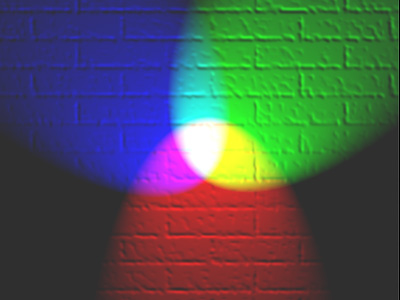
\includegraphics[width=0.4\textwidth]{RGBillumination.png}
    \caption{Hojas bajo distintas iluminaciones.\footfullcite{RGBillumination}}
  \end{figure}
  \end{exampleblock}

\end{frame}
%--- Next Frame ---%

\section{Firmas espectrales}
\begin{frame}{Reflectancia}
  Queremos calcular el cociente de la radiancia saliente de una cobertura sobre la radiancia incidente. \pause
  \begin{block}{Definición}
    Definimos la \emph{BRDF} (espectral bidirectional reflectance distribution function) como:
    \begin{equation}
          f(\theta_i, \phi_i, \theta_r, \phi_r) = \frac{dL(\theta_i, \phi_i, \theta_r, \phi_r)}{dE(\theta_i, \phi_i)}
    \end{equation}
  \end{block}
\end{frame}
%--- Next Frame ---%

\begin{frame}{Reflectancia}
  \begin{block}{Definición}
    Definimos la reflectancia direccional como:
    \begin{equation}
     R(\theta_i, \phi_i, \theta_r, \phi_r) = \frac{\pi L(\theta_i, \phi_i, \theta_r, \phi_r)}{\cos(\theta_i) E_0} = \pi f(\theta_i, \phi_i, \theta_r, \phi_r)
    \end{equation}
    Donde $\theta$ y $\phi$ son los ángulos zenitales y azimutales respectivamente.
  \end{block}
\end{frame}
%--- Next Frame ---%

\begin{frame}{Reflectancia direccional}
  \begin{exampleblock}{Ejemplo}
    \begin{figure}
      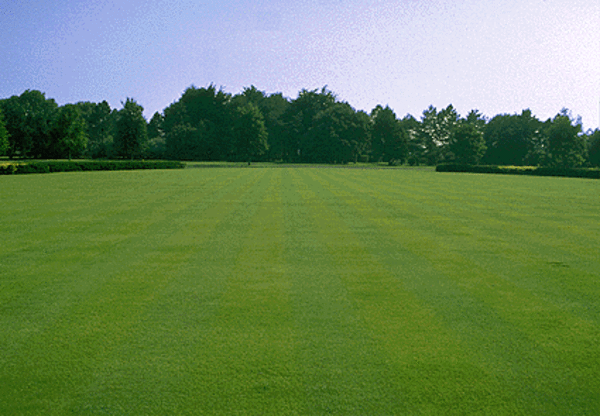
\includegraphics[width=0.6\textwidth]{grass.png}
      \caption{Un parque.\footfullcite{grass}}
    \end{figure}
  \end{exampleblock}
\end{frame}

\begin{frame}{Reflectancia direccional}
  \begin{exampleblock}{Ejemplo}
    \begin{figure}
      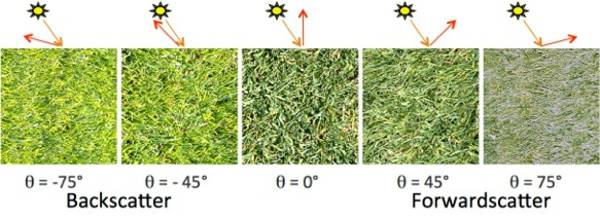
\includegraphics[width=0.6\textwidth]{grass2.png}
      \caption{Pasto bajo distintas iluminaciones.\footfullcite{grass}}
    \end{figure}
  \end{exampleblock}
\end{frame}

%--- Next Frame ---%
\begin{frame}{Reflectancia direccional}
  \begin{exampleblock}{Ejemplo}
    \begin{figure}
      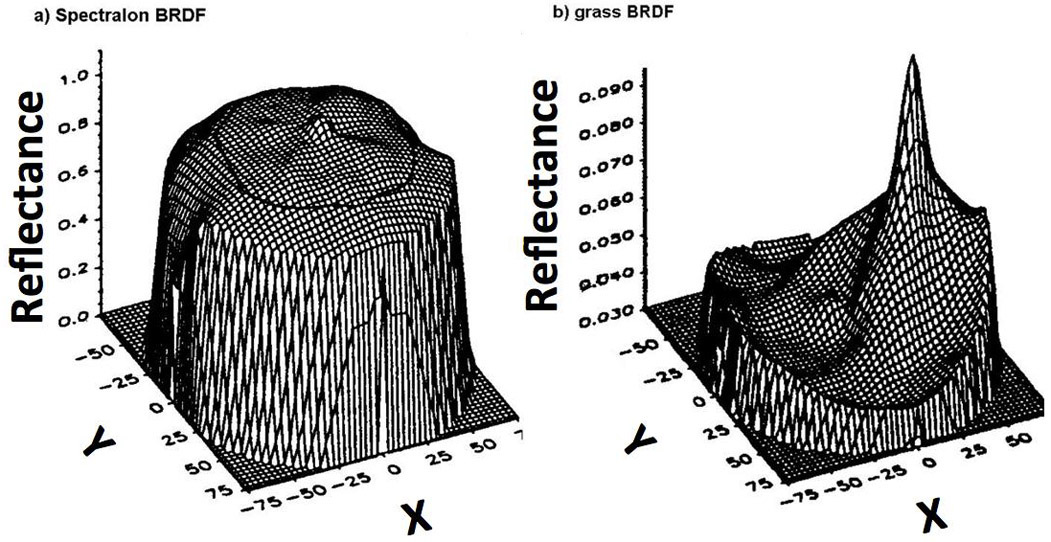
\includegraphics[width=0.6\textwidth]{grass_brdf.png}
      \caption{Reflectancia del pasto en función del ángulo zenital y asimutal.\footfullcite{clark2014passive}}
    \end{figure}
  \end{exampleblock}
\end{frame}
%--- Next Frame ---%


%--- Next Frame ---%
\begin{frame}{Reflectancia direccional}
  \begin{figure}
    \includegraphics[width=0.6\textwidth]{reflectancias.png}
    \caption{En general podemos clasificar la reflectancia en función de que tan fuertemente depende del ángulo.}
  \end{figure}
\end{frame}
%--- Next Frame ---%

\begin{frame}{Aproximaciones}
  \begin{block}{Definición}
    Hablamos de la aproximación \emph{especular} cuando la reflectancia es una delta del ángulo.
  \end{block}\pause
  \begin{block}{Definición}
    Hablamos de la aproximación \emph{lambertiana} cuando la reflectancia no depende del ángulo.
  \end{block}
\end{frame}

\begin{frame}{Aproximaciones}
  \begin{alertblock}{Importante}
    En el curso vamos a trabajar en la aproximación Lambertiana. Esto es solo una aproximación que simplifica y mucho el problema.
  \end{alertblock}
\end{frame}
%--- Next Frame ---%

\begin{frame}{Reflectancia}
  \begin{block}{Definición}
    En la aproximación lambertiana defininos la \emph{reflectancia} como
    \begin{equation}
      \rho = \frac{\pi L}{\cos \theta_z E_0}
    \end{equation}
  \end{block}
\end{frame}

\begin{frame}{Aproximaciones}
  \begin{alertblock}{Importante}
    La reflectancia depende solo de la superficie que estamos mirando.
  \end{alertblock}
\end{frame}
%--- Next Frame ---%

\end{document}
